
\section{Experiment=28: Drip tectonics}

The setup is based on \fullcite{gops17}.
The setup information is presented in the paper and in its appendix. 

``The numerical code employed here, SOPALE, uses arbitrary
Lagrangian–Eulerian (ALE) finite element techniques to solve for the plane-strain
deformation of complex visco-plastic materials. The ALE technique is useful for
treating finite deformations, and for tracking boundaries (surface and Moho
topography) and internal particles ($P-T$ paths). The configuration of the
model is designed as a general representation for the gravitationally unstable arc
root removal from beneath the crust into the mantle.''

``Forward geodynamical models explore the
dynamics and the tectonic response to the removal of $\sim$280 km
wide $\times$ 160 km thick (25\% thickened), gravitationally unstable
lithosphere as an approximation to the foundering of Kırşehir arc
root (sub-arc mantle lithosphere) after thickening.'' 

``
In these models, density, $\rho$, is a function of composition and
temperature, $\rho = \rho_0 (1–\alpha (T-T_0))$, 
where $T$ is temperature, $\alpha = 2 \times 10^{-5}\si{\per\kelvin}$ is the coefficient of 
thermal expansion, $T_0 = 25\si{\degree}$ is
the reference temperature, and $\rho_0$ is the reference density that
depends on material. [...]

For rheological calculations we use laboratory measurements
based on a viscous flow law of 
$\dot\varepsilon = A \sigma^n \exp (-Q/RT)$. 
Here, $\dot\varepsilon$ strain rate, $T$ is temperature, $\sigma$ 
is deviatoric stress, and the
variables $A$, $n$, $Q$, and $R$ are the viscosity parameter, power law
exponent, activation energy, and ideal gas constant, respectively.

The EXP-1 (preferred model) uses the temperature-independent
mantle lithosphere rheology with viscous flow law parameters
$Q=0$ and $A=10^{-38}\si{\pascal}^{-n}\si{\per\second}$. Based on strain rates of $10^{-12}$ to
$10^{-17}\si{\per\second}$ that are characteristic of flow in the models, this
corresponds to the mantle lithosphere viscosity $\mu$ at the sub-arc
region and elsewhere in the model ranging from $2.69 \times 10^{19}$ to
$5 \times 10^{23}\si{\pascal\second}$. For the practical purpose in these calculations we set
the minimum and maximum viscosity variation ranging from
$5\times 10^{19}$ to $5 \times 10^{22}\si{\pascal\second}$.
{\color{red} why this specific range?}



\begin{center}
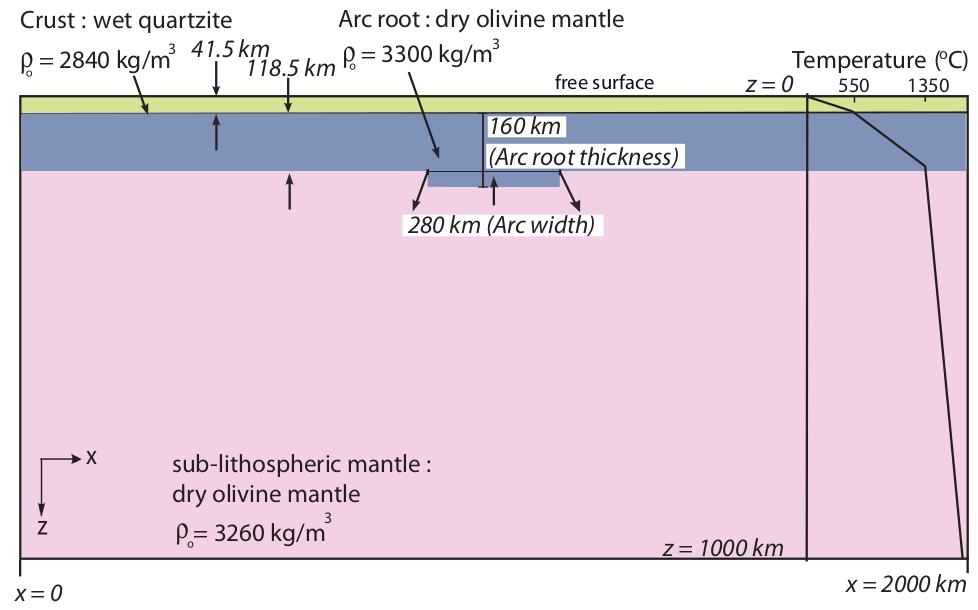
\includegraphics[width=12cm]{exp28/gops17a}
\end{center}

``In the models, the 160 km thick lithosphere is made up of 41.5 km thick crust 
($\rho_0=2840\si{\kg\per\cubic\meter}$, yellow) 
and 118.5 km thick mantle lithosphere ($\rho_0=3300\si{\kg\per\cubic\meter}$, blue) 
overlying a sub-lithospheric mantle region ($\rho_0=3260\si{\kg\per\cubic\meter}$, pink). 
The width (280 km) and the thickness (160 km) of the arc root instability are based on geological 
and paleomagnetic studies on the Late Cretecaus\footnote{did nobody proofread this paper?!} 
granitoids of Central Anatolia.''
{\color{red} it looks like there is a taper on the thickened region? I need to ask him.}

\begin{center}
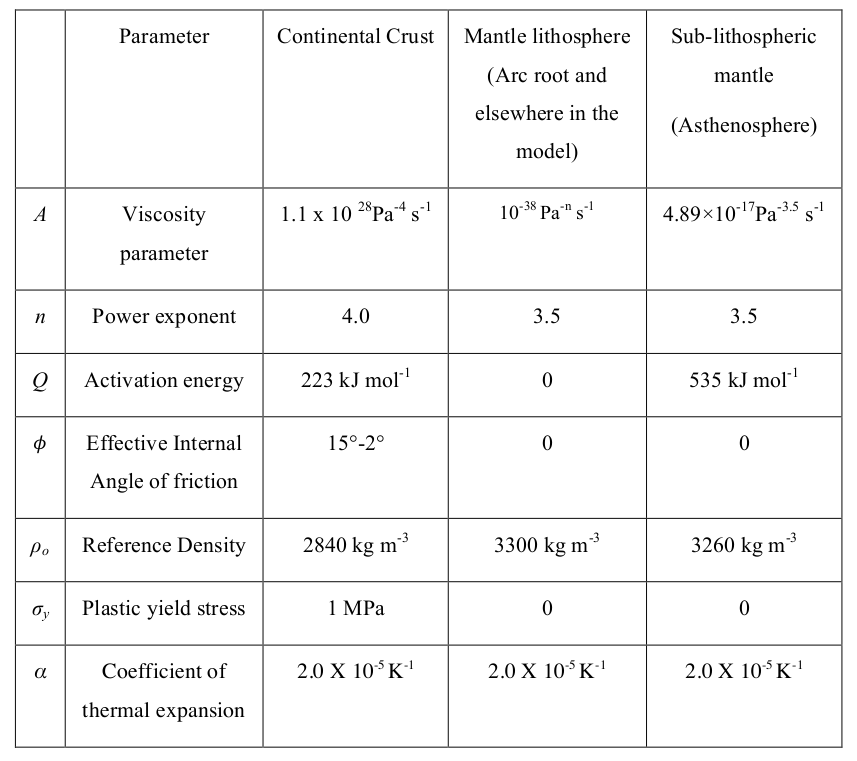
\includegraphics[width=11cm]{exp28/gops17b}
\end{center}


``The numerical (width) and (depth) resolution is $201 \times 101$ Eulerian nodes
\footnote{so 200x100 Q1P0 elements} and
$601 \times 301$ Lagrangian nodes. Half of the Eulerian and Lagrangian elements are
concentrated in the top 160 km in order to enhance resolution in the lithosphere.
The model has a free top surface, allowing topography to develop as the model
evolves. The mechanical boundary conditions at the other three sides are defined
by zero tangential stress and normal velocity (e.g., free slip). We have extended
the depth of the solution space into the lower mantle so that the sinking mantle
lithosphere material moves away from the lithosphere\footnote{Seriously? the 660, which 
would slow down the drip has just been removed?!}. The initial geotherm for the
experiments is laterally uniform and is defined by a surface temperature of $25\si{\celsius}$,
an increase to 550\si{\celsius} at the Moho, an increase to 1350\si{\celsius} at the base of the mantle
lithosphere, and an increase to 1525\si{\celsius} at the bottom of the model. 
[...]
The surface and bottom temperatures are held constant throughout the
experiments and the heat flux across the side boundaries is zero. The initial
temperature profile is the same in all experiments. Thermal properties (thermal
conductivity $k = 2.25\si{\watt\per\meter\per\kelvin}$, 
heat capacity $C_p= 1250\si{\joule\per\kg\per\kelvin}$) are the same
for all materials and we ignore radioactive heat production and shear heating in the
model. In this work we do not take into account explicitly petrological processes of
decompression and/or hydrated mantle melting.''

{\color{red} Although the paper uses ALE for free surface, I want to start with free slip on all four sides.}

{\color{red} at the moment no strain weakening} 


The initial temperature is then as follows:


\begin{lstlisting}
def initial_temperature(x, z, rad, theta, nn_V):
    z3 = 1000e3
    z2 = 1000e3 - 41.5e3
    z1 = 840e3
    z0 = 0
    T3 = 25 + 273
    T2 = 550 + 273
    T1 = 1350 + 273
    T0 = 1525 + 273
    for ip in range(0, nn_V):
        if z[ip] <= z1:   T[ip] = (z[ip] - z0) / (z1 - z0) * (T1 - T0) + T0
        elif z[ip] <= z2: T[ip] = (z[ip] - z1) / (z2 - z1) * (T2 - T1) + T1
        elif z[ip] <= z3: T[ip] = (z[ip] - z2) / (z3 - z2) * (T3 - T2) + T2
\end{lstlisting}

{\color{red} I have a question: should temperature geotherm follow the bottom thickened listhosphere?}

and the material layout is implemented as follows:


\begin{lstlisting}
def particle_layout(nparticle, nmat, swarm_x, swarm_z, swarm_rad, swarm_theta, Lx, Lz):
    for ip in range(0, nparticle):
        if swarm_z[ip] >= Lz - 41.5e3:  # crust
            swarm_wf[0, ip] = 1
        elif swarm_z[ip] >= Lz - 160e3 and swarm_z[ip] < Lz - 41.5e3:  # arc root
            swarm_wf[1, ip] = 1
        elif abs(swarm_x[ip] - Lx / 2) < 140e3 and swarm_z[ip] >= Lz - 201.5e3 and swarm_z[ip] < Lz - 160e3:  # arc root
            swarm_wf[1, ip] = 1
        else:  # mantle
            swarm_wf[2, ip] = 1
    return swarm_wf, material_names
\end{lstlisting}




%\newpage
\begin{center}
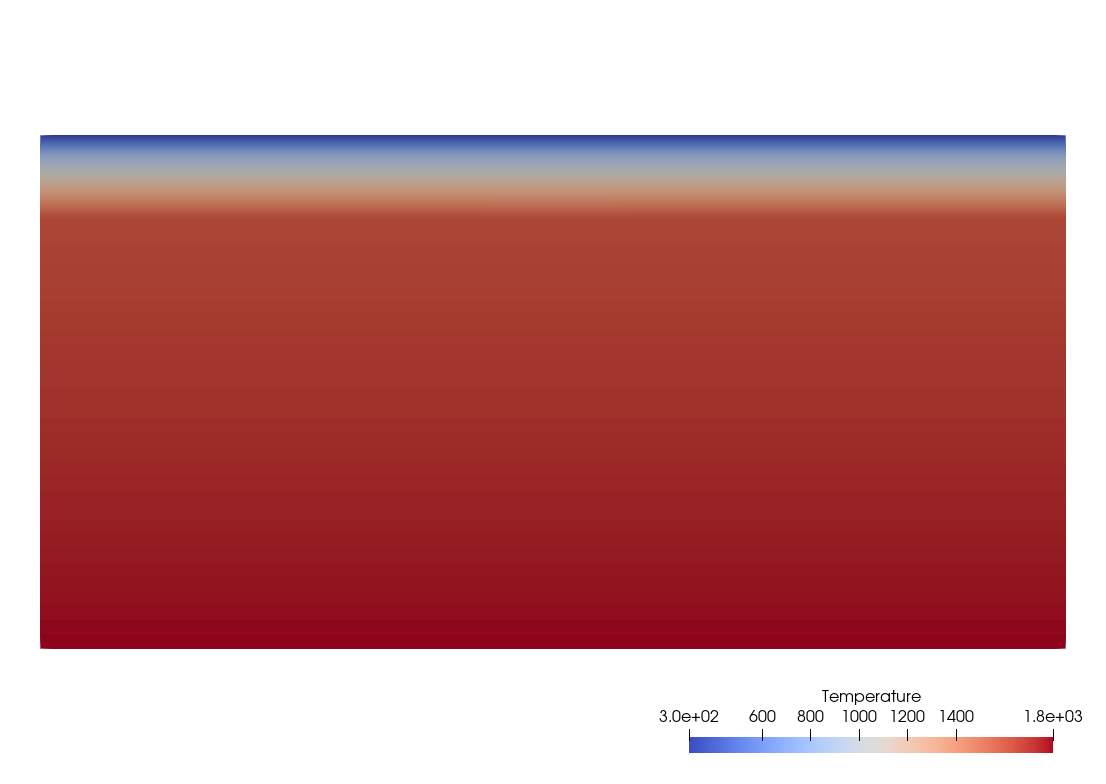
\includegraphics[width=8cm]{exp28/temperature}
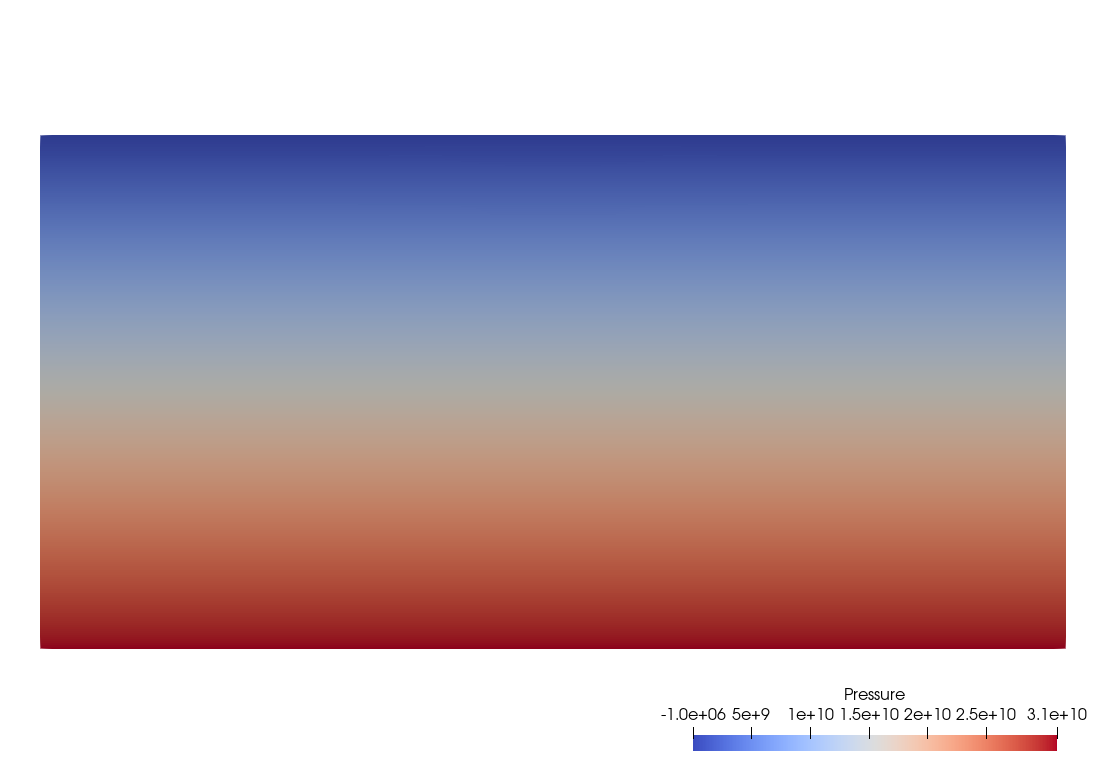
\includegraphics[width=8cm]{exp28/pressure}\\
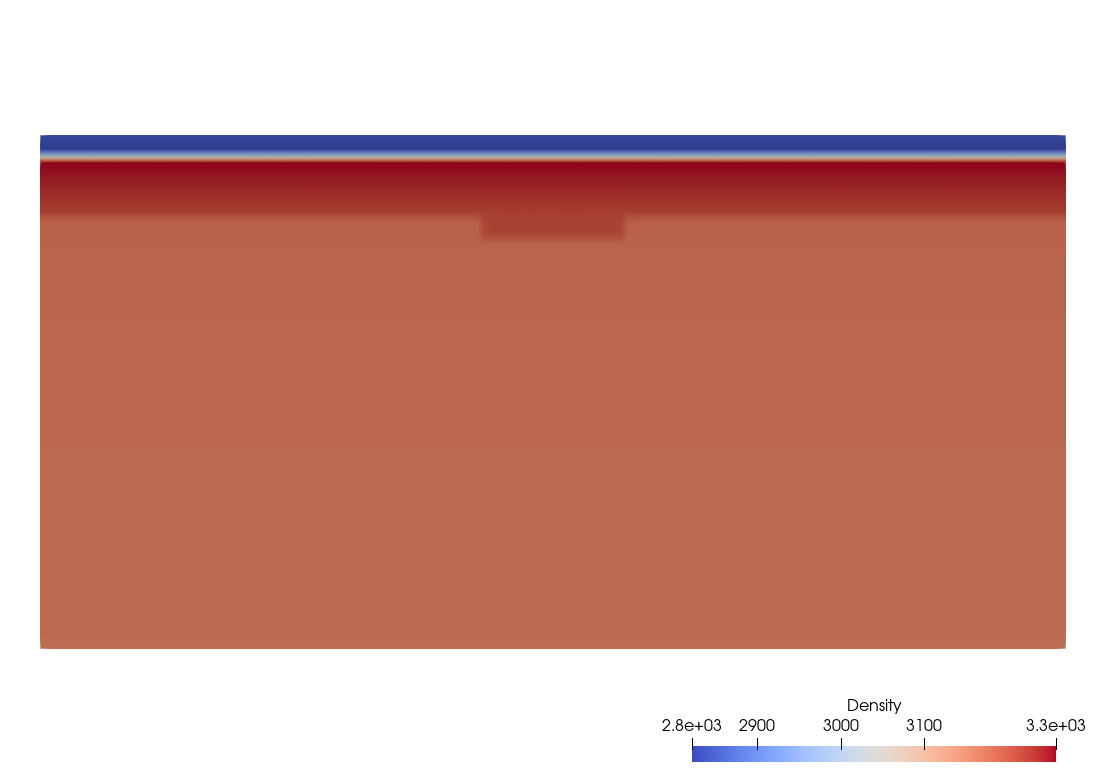
\includegraphics[width=8cm]{exp28/density}

\includegraphics[width=8cm]{exp28/vel}\\
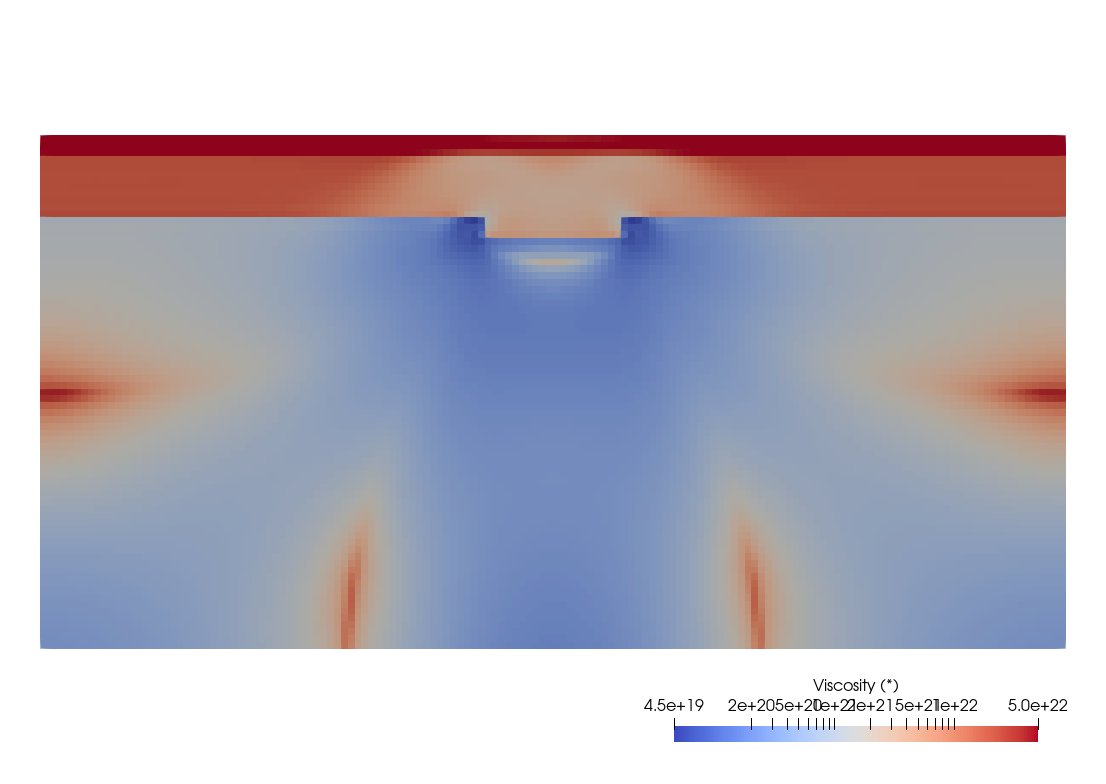
\includegraphics[width=8cm]{exp28/viscosity}
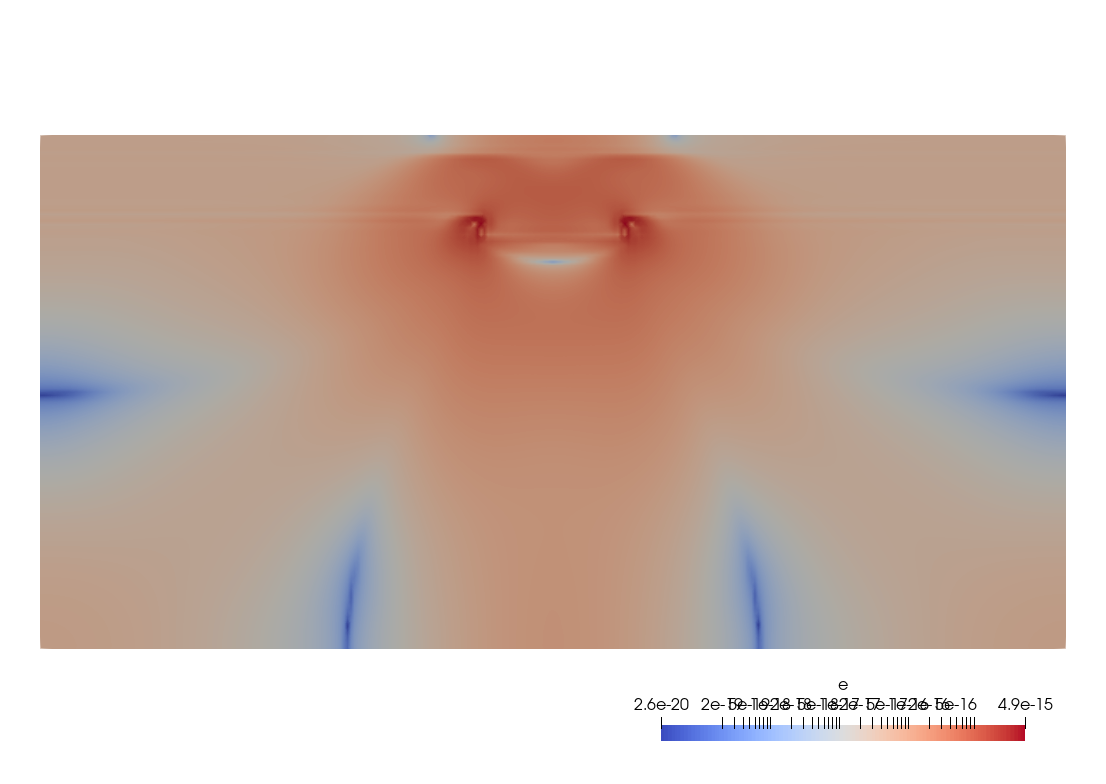
\includegraphics[width=8cm]{exp28/strainrate}\\
Obtained on 128x64 mesh at the end of the first time step (20 nonlinear iterations), 
100 ptcls per element, harmonic averaging for viscosity.
\end{center}
